\section{Тренировочное задание}

Вариант: 1

Задачи:
\begin{enumerate}
	\item Дополнить временной план проекта, подготовленный на предыдущем этапе (лабораторная работа № 1), информацией о ресурсах и определить стоимость проекта.
	\item Для этого заполнить ресурсный лист в программе MS Project, принимая во внимание, что к реализации проекта привлекается не более 11 исполнителей.
	\item Предусмотреть, что стандартная ставка ресурса составляет 120 руб./день.
	\item Произвести назначение ресурсов на задачи в соответствии с таблицей \ref{fig:task01} С учетом того, что квалификация ресурсов одинаковая, при назначении ресурсов использовать процент загрузки.
\end{enumerate}

\begin{figure}[H]
	\centering
	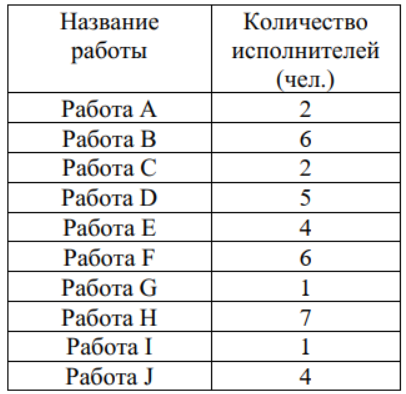
\includegraphics[width=0.7\linewidth]{task0_1}
	\caption{}
	\label{fig:task01}
\end{figure}

Призаданных условиях стоимость проекта составляет: 35805.71р, но силами 11 программистов сделать данный проект, при указанных условиях, невозможно (Смотрите изображение \ref{fig:task04}). Для выхода из данной ситуации есть несколько вариантов:
\begin{enumerate}
	\item Увеличить состав программистов (Не подходит по условиям задачи. Макс 11);
	\item Сдвинуть план с целью распределения \ref{fig:task03}.
\end{enumerate}

\begin{figure}[H]
	\centering
	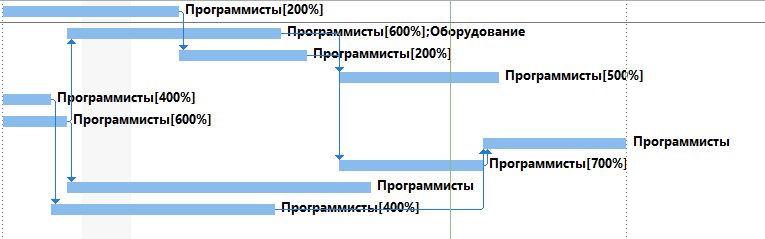
\includegraphics[width=0.7\linewidth]{src/task0_4}
	\caption{Изначальные сроки}
	\label{fig:task04}
\end{figure}
\begin{figure}[H]
	\centering
	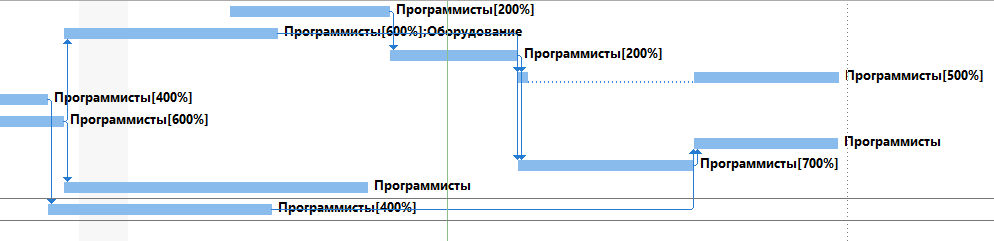
\includegraphics[width=0.7\linewidth]{src/task0_3}
	\caption{Обновленные}
	\label{fig:task03}
\end{figure}

\section{Задание 1}
Заполнить ресурсный лист в соответсвии с таблицей. Результат заполнения указан на изображении \ref{fig:task11}

\begin{figure}[H]
	\centering
	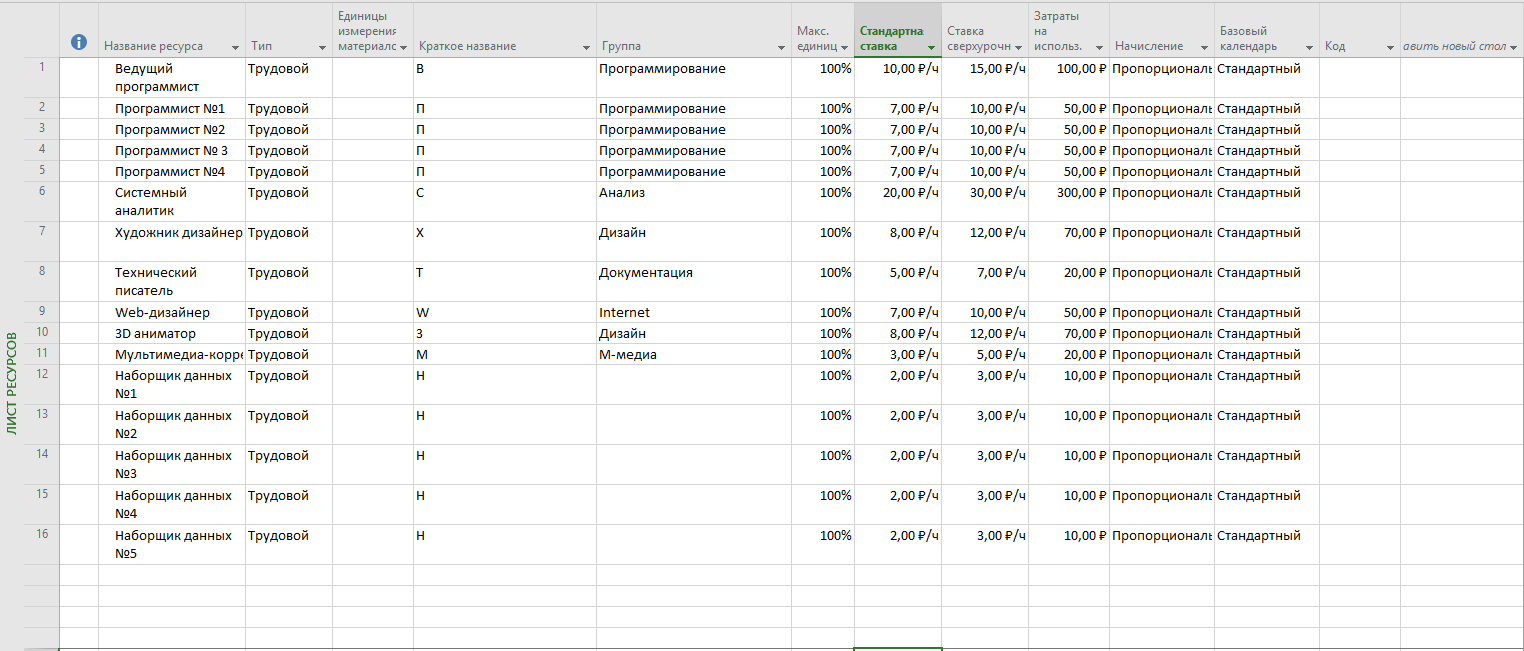
\includegraphics[width=0.7\linewidth]{src/task1_1}
	\caption{Заполненная таблица ресурсов}
	\label{fig:task11}
\end{figure}

На изображениях \ref{fig:task12}, \ref{fig:task13} отображен процесс заполнения информации о ресурсах.

\begin{figure}[H]
	\centering
	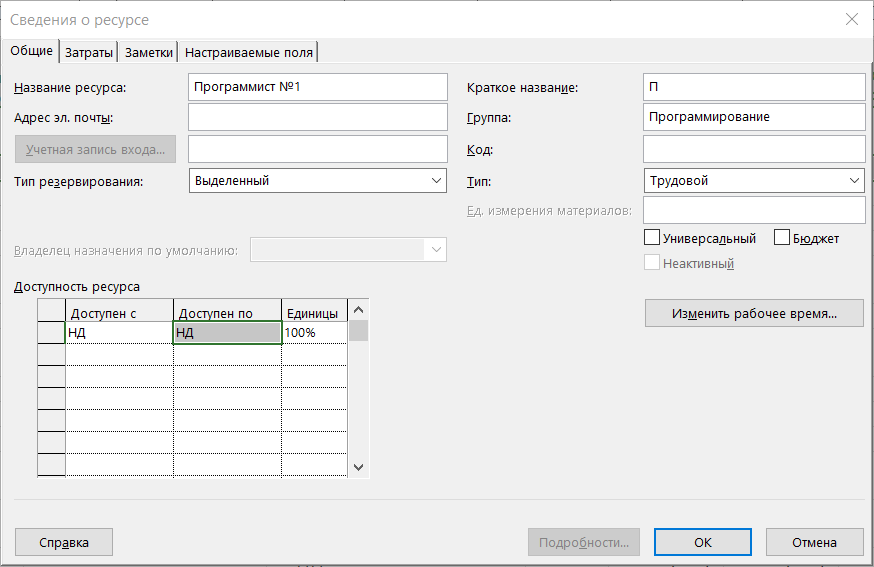
\includegraphics[width=0.7\linewidth]{src/task1_2}
	\caption{Заполнение информации по ресурсу}
	\label{fig:task12}
\end{figure}

\begin{figure}[H]
	\centering
	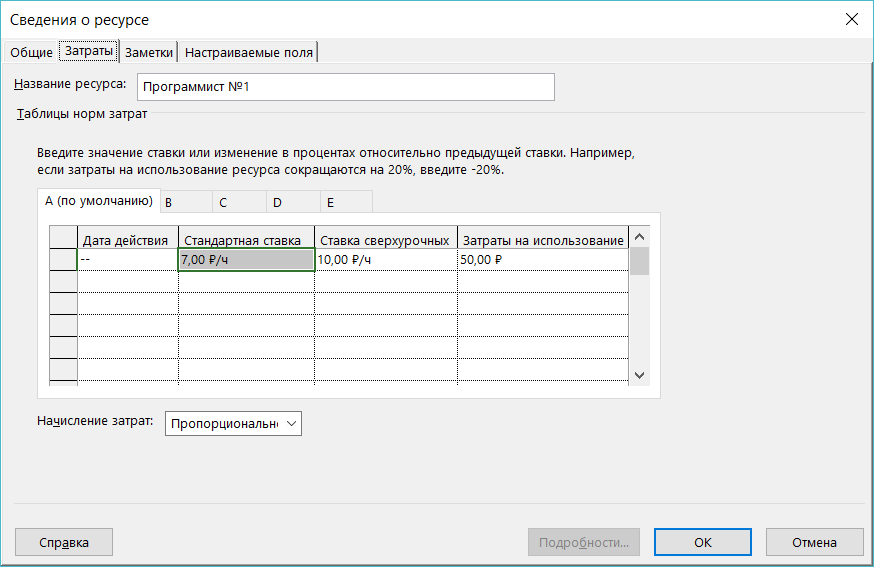
\includegraphics[width=0.7\linewidth]{src/task1_3}
	\caption{Заполнение затрат}
	\label{fig:task13}
\end{figure}

\section{Задание 2}
Подзадачи:
\begin{enumerate}
	\item Назначить ресурсы задачам в соответсвии с таблицей;
	Для этого в таблице выбираем необходимую нам задачу и в контекстном меню выбираем "Назначение ресурсов" (смотри изображение \ref{fig:task21}) или в с столбце "Названия ресурсов" выбираем небходимые ресурсы;
	\item Задайте задачам 2,8 и 12 по 1000р фиксированных затрат. Для этого в представлении "Диаграмма Ганта" выберем Вид -> Таблица -> Завтра вместо Вид -> Таблицы -> Запись (Смотрите изображение \ref{fig:task35}).
	\item Арендуйте для задачи N8 "Построение базы объектов" дополнительный сервер. Стоимость аренды - 2 ребля в час. Для этого создадим ресур "Аренда сервера".
\end{enumerate}

\begin{figure}[H]
	\centering
	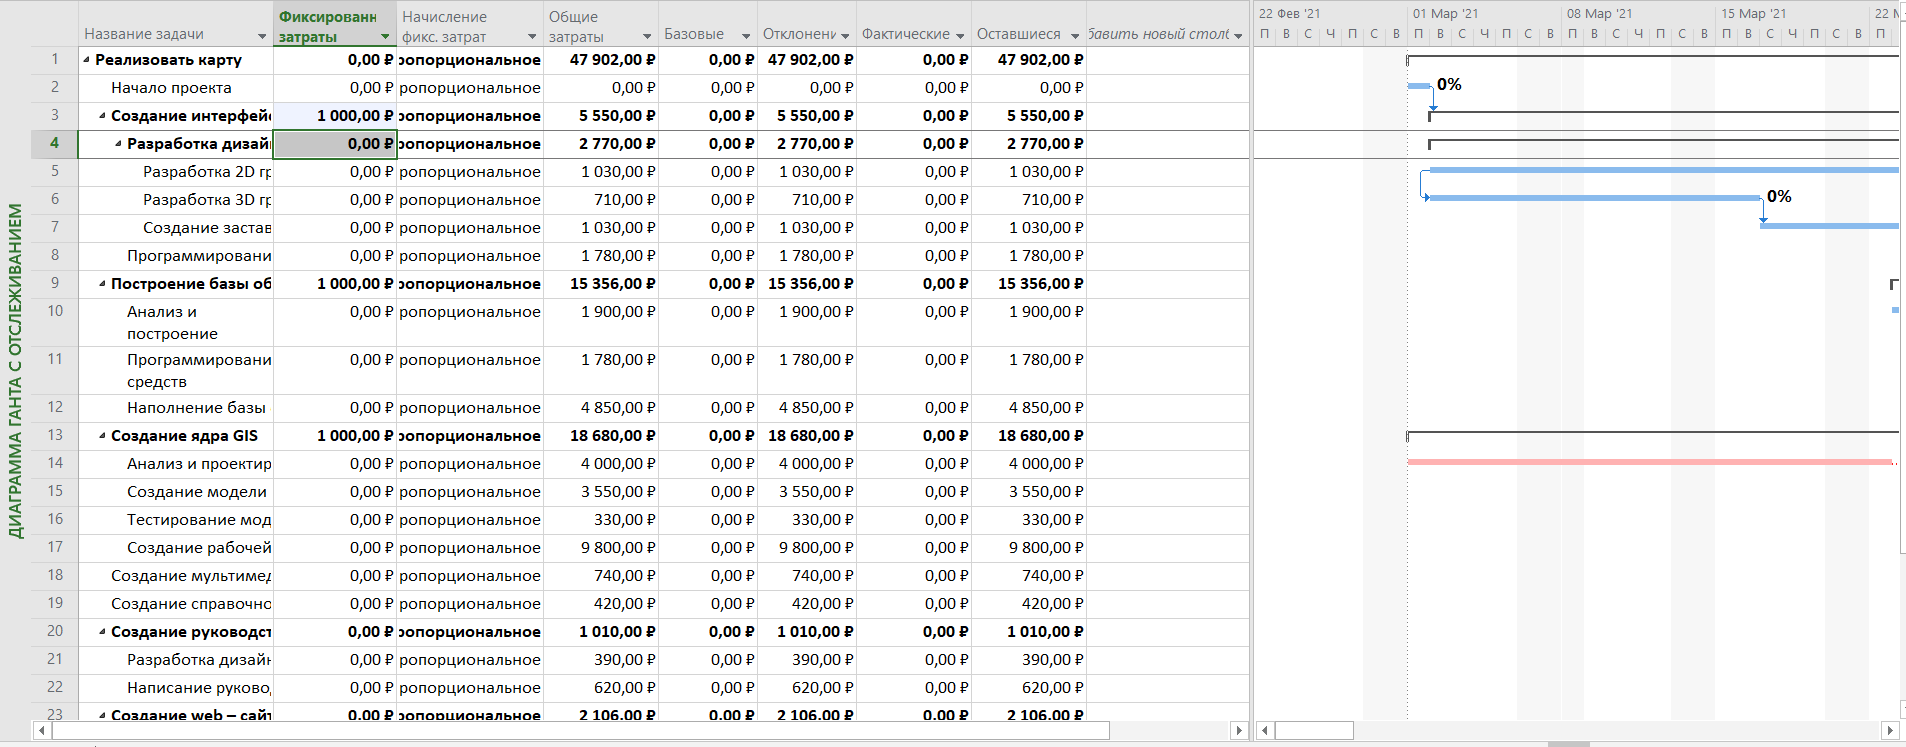
\includegraphics[width=0.7\linewidth]{src/task3_5}
	\caption{Назначение ресурсов задачам}
	\label{fig:task35}
\end{figure}


\begin{figure}[H]
	\centering
	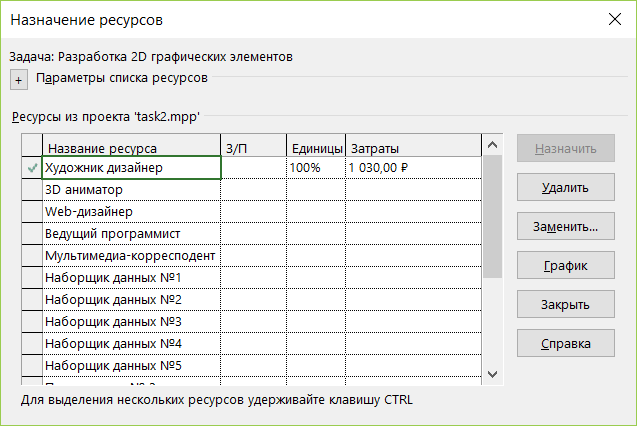
\includegraphics[width=0.7\linewidth]{src/task2_1}
	\caption{Назначение ресурсов}
	\label{fig:task21}
\end{figure}

\section{Задание 3}
Подзадачи:
\begin{enumerate}
	\item Проведите структуризация затрат по группам ресурсов;
	\item Информацию о затратах по структурным группам ресурсов представьте в
	графическом виде;
	\item Выполните структуризацию трудозатрат по тем же группам ресурсов,
	представив результат так же в графической форме;
	\item Проведите сопоставление в логике «Деньги» – «Объем работ» и сделайте
	выводы по результатам проведенного анализа.
\end{enumerate}

На основе групп ресурсов был сформулирован отчет, представленный диаграммами и таблицами (\ref{fig:task31}, \ref{fig:task32}, \ref{fig:task33}, \ref{fig:task34},
\ref{fig:task35})

\begin{figure}[H]
	\centering
	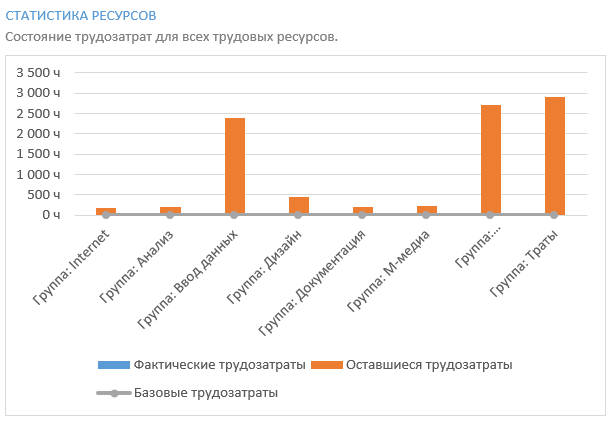
\includegraphics[width=0.7\linewidth]{src/task3_1}
	\caption{}
	\label{fig:task31}
\end{figure}
\begin{figure}[H]
	\centering
	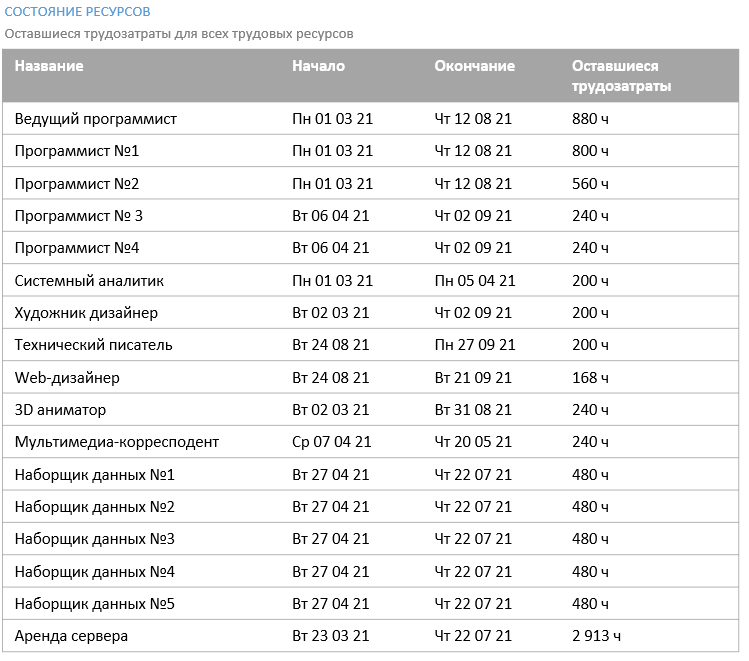
\includegraphics[width=0.7\linewidth]{src/task3_2}
	\caption{}
	\label{fig:task32}
\end{figure}
\begin{figure}[H]
	\centering
	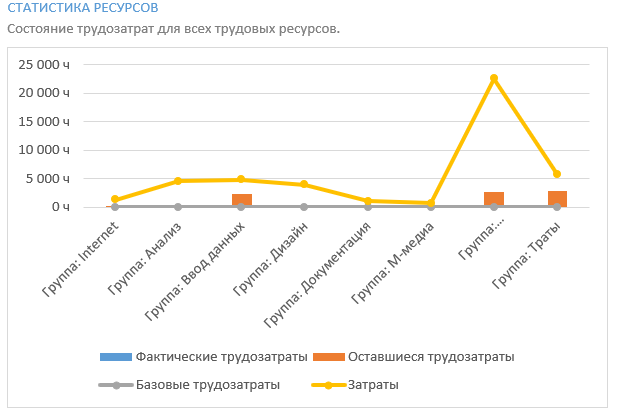
\includegraphics[width=0.7\linewidth]{src/task3_3}
	\caption{}
	\label{fig:task33}
\end{figure}
\begin{figure}[H]
	\centering
	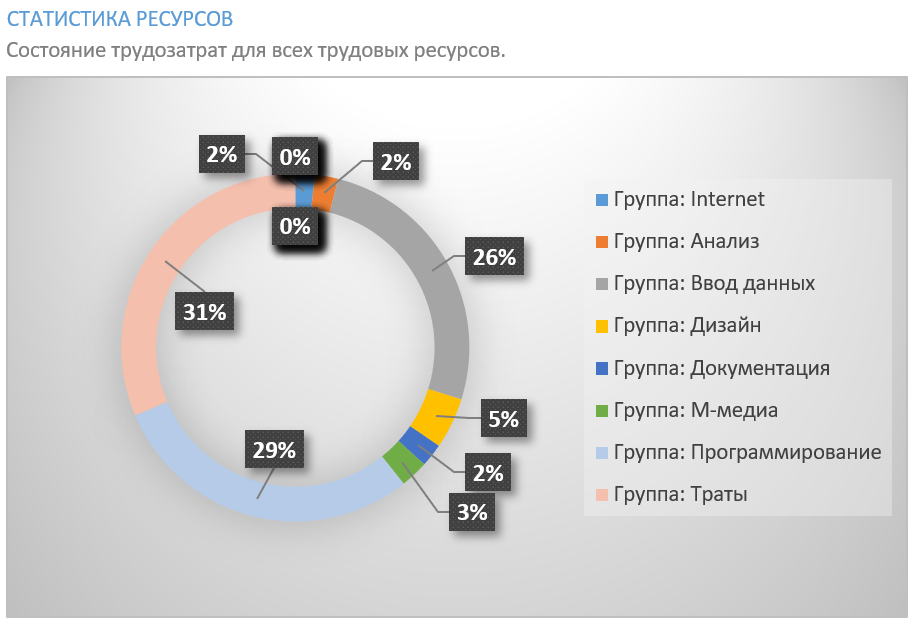
\includegraphics[width=0.7\linewidth]{src/task3_4}
	\caption{}
	\label{fig:task34}
\end{figure}

Суммарные трудозатраты на проект составляет 47902 рубля, что укладывается в бюджет проекта, составляющий 5000рублей (смотрите изображение \ref{fig:task35}).

\begin{figure}[H]
	\centering
	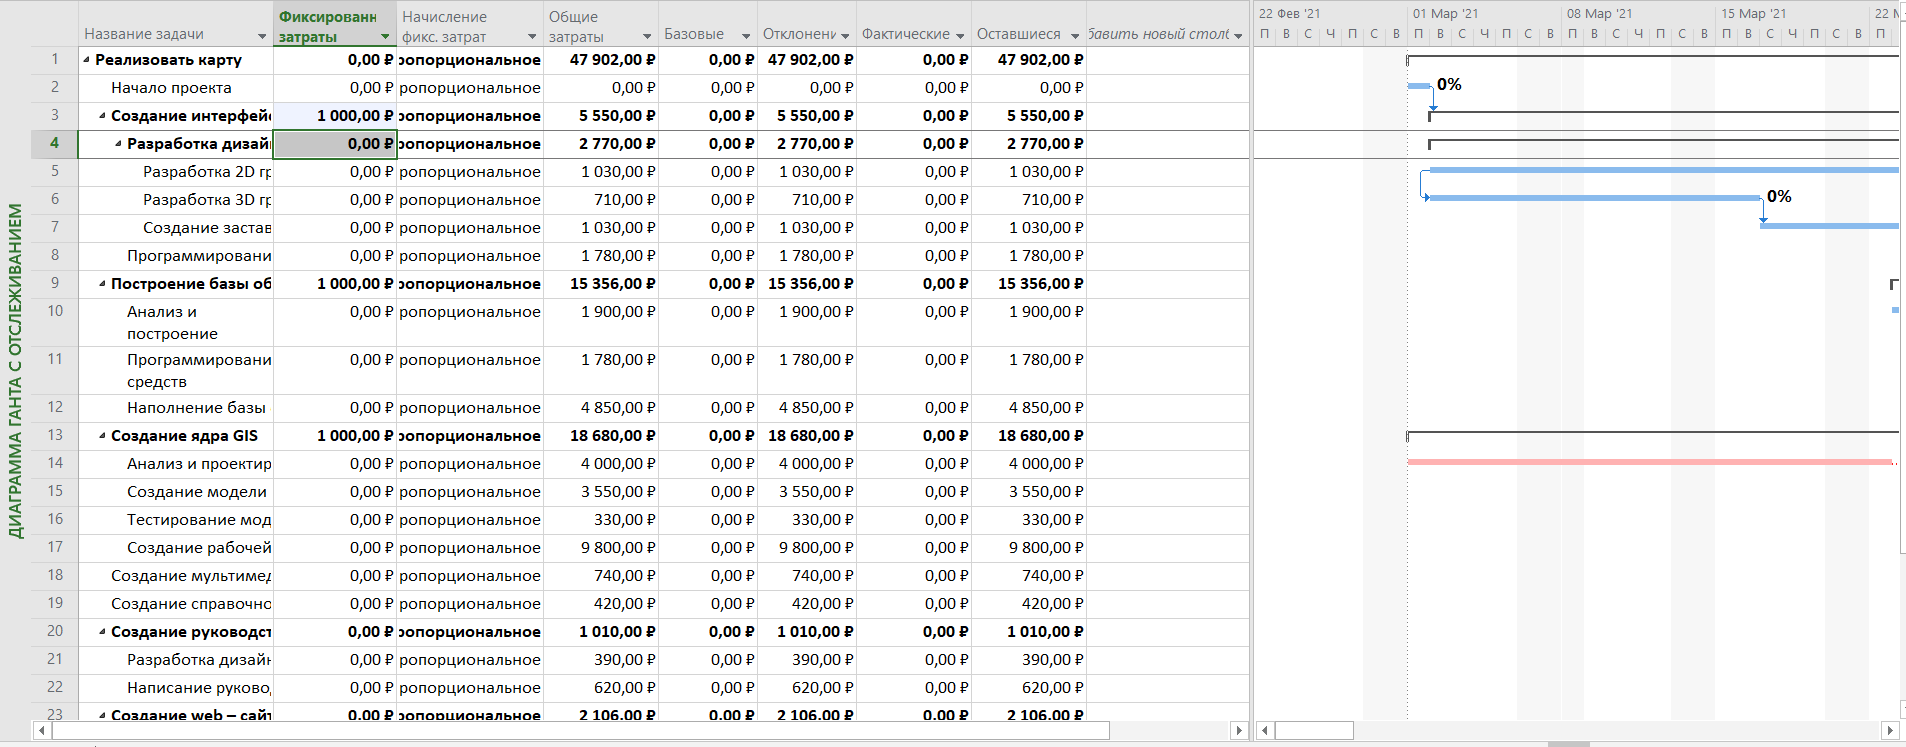
\includegraphics[width=0.7\linewidth]{src/task3_5}
	\caption{Траты}
	\label{fig:task35}
\end{figure}

\section{Вывод}
При выполнении лабораторной работы удалось ознакомиться с возможностями программы Microsoft Project для соотнесения ресурсов (людей требуемых профессий и дополнительного сервера для одной из задач) и задач.

При этом в результате выполнения работы Microsoft Project выводил к некоторым задачам следующее предупреждение: «Задача содержит ресурсы с превышением доступности». Такое предупреждение было выведено для задач 9, 13, 18, 20, 21 и 24.

Такое предупреждение выводилось для ситуаций, когда один и тот же ресурс используется одновременно в нескольких задачах. Например, такая ситуация возникает для задач 9 и 13 с ресурсом «Системный аналитик». Поскольку предполагается, что один человек не сможет работать одновременно над двумя задачами на полную ставку, Microsoft Project автоматически фиксирует эту проблему, выводит предупреждение и предлагает перезапланировать одну из задач с совпавшим ресурсом на другой срок выполнения.

Из рисунке \ref{fig:task34} видно, что наиболее значительные суммы расходов составляют следующие группы расходов:

1) оплата дополнительного сервера;

2) заработная плата программистов.

При этом суммарный рассчитанный бюджет (47950 рубля) укладывается в запланированный в проекте.











